%% GENERATED by scripts/make_figure1.py -- edit the generator, not this file.
\documentclass[border=6pt]{standalone}
\usepackage{tikz}
\usetikzlibrary{arrows.meta}
\usepackage{sansmath}
\renewcommand{\familydefault}{\sfdefault}
\sansmath
\definecolor{ink}{HTML}{1B2430}
\definecolor{inkdim}{HTML}{5D7185}
\definecolor{gridc}{HTML}{C9D3DE}
\definecolor{sph}{HTML}{D9DEE4}
\definecolor{sub}{HTML}{C8CED6}
\definecolor{shellc}{HTML}{EEF1F5}
\definecolor{uhi}{HTML}{1D3A7A}
\definecolor{ulo}{HTML}{F5DFA0}
\definecolor{spA}{HTML}{1D3A7A}
\definecolor{spB}{HTML}{A4C639}
\definecolor{spAB}{HTML}{2BB3A3}
\tikzset{
  gridl/.style={draw=gridc, line width=0.5pt},
  gridb/.style={draw=gridc!70!ink, line width=0.6pt},
  shell/.style={fill=shellc},
  op/.style={-{Stealth[length=7pt,width=5pt]}, line width=1.4pt, ink},
  mv/.style={-{Stealth[length=4pt,width=3.5pt]}, line width=0.9pt, ink},
  gen/.style={-{Stealth[length=5pt]}, line width=0.9pt, inkdim},
  lbl/.style={font=\small, ink},
  reads/.style={-{Stealth[length=5pt]}, line width=0.9pt, inkdim, dashed},
}
\newcommand{\num}[1]{\tikz[baseline=(n.base)]\node[draw=ink, circle, line width=0.6pt, inner sep=0.8pt, font=\scriptsize](n){#1};}
\begin{document}
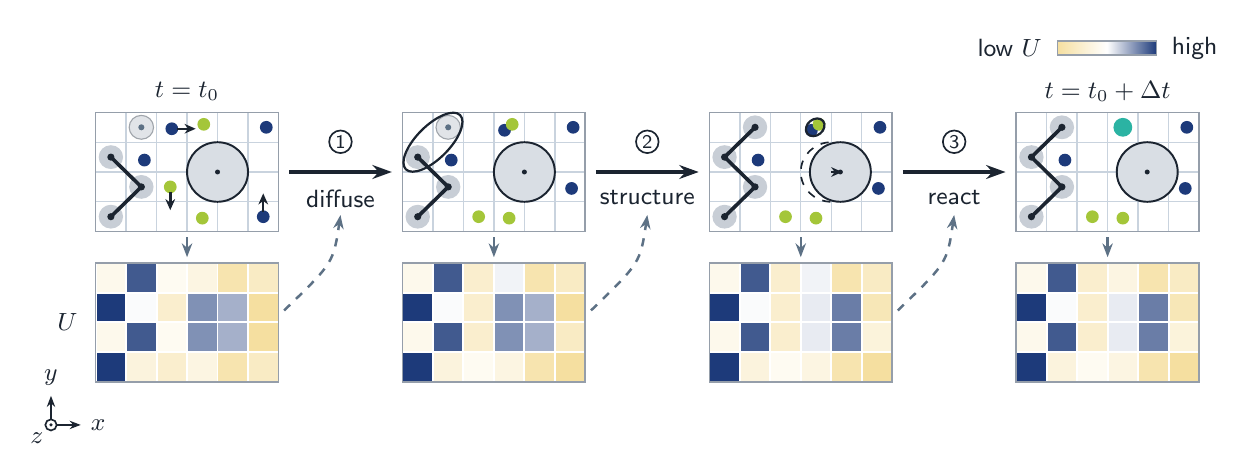
\begin{tikzpicture}[x=0.9cm, y=0.88cm]
\draw[gridl, shift={(0.830,-1.950)}] (0,0) grid[step=0.430] (2.580,1.720);
\draw[gridb] (0.830,-1.950) rectangle (3.410,-0.230);
\fill[sph, draw=ink, line width=0.7pt] (2.550,-1.090) circle (0.430);
\fill[ink] (2.550,-1.090) circle (0.9pt);
\fill[sub] (1.045,-1.735) circle (0.172);
\fill[sub] (1.475,-1.305) circle (0.172);
\fill[sub] (1.045,-0.875) circle (0.172);
\fill[sub!55!white, draw=sub!80!black, line width=0.4pt] (1.475,-0.445) circle (0.172);
\fill[inkdim] (1.475,-0.445) circle (1.1pt);
\draw[ink, line width=1.3pt] (1.045,-1.735) -- (1.475,-1.305) -- (1.045,-0.875);
\fill[ink] (1.045,-1.735) circle (1.3pt);
\fill[ink] (1.475,-1.305) circle (1.3pt);
\fill[ink] (1.045,-0.875) circle (1.3pt);
\fill[spA] (1.905,-0.466) circle (2.3pt);
\fill[spB] (2.356,-0.402) circle (2.3pt);
\fill[spA] (3.195,-1.735) circle (2.3pt);
\fill[spB] (1.883,-1.305) circle (2.3pt);
\fill[spA] (3.238,-0.445) circle (2.3pt);
\fill[spB] (2.335,-1.756) circle (2.3pt);
\fill[spA] (1.518,-0.918) circle (2.3pt);
\draw[gen] (2.120,-2.030) -- (2.120,-2.320);
\draw[gridl, shift={(5.160,-1.950)}] (0,0) grid[step=0.430] (2.580,1.720);
\draw[gridb] (5.160,-1.950) rectangle (7.740,-0.230);
\fill[sph, draw=ink, line width=0.7pt] (6.880,-1.090) circle (0.430);
\fill[ink] (6.880,-1.090) circle (0.9pt);
\fill[sub] (5.375,-1.735) circle (0.172);
\fill[sub] (5.805,-1.305) circle (0.172);
\fill[sub] (5.375,-0.875) circle (0.172);
\fill[sub!55!white, draw=sub!80!black, line width=0.4pt] (5.805,-0.445) circle (0.172);
\fill[inkdim] (5.805,-0.445) circle (1.1pt);
\draw[ink, line width=1.3pt] (5.375,-1.735) -- (5.805,-1.305) -- (5.375,-0.875);
\fill[ink] (5.375,-1.735) circle (1.3pt);
\fill[ink] (5.805,-1.305) circle (1.3pt);
\fill[ink] (5.375,-0.875) circle (1.3pt);
\fill[spA] (6.600,-0.488) circle (2.3pt);
\fill[spB] (6.708,-0.402) circle (2.3pt);
\fill[spA] (7.546,-1.327) circle (2.3pt);
\fill[spB] (6.235,-1.735) circle (2.3pt);
\fill[spA] (7.568,-0.445) circle (2.3pt);
\fill[spB] (6.665,-1.756) circle (2.3pt);
\fill[spA] (5.848,-0.918) circle (2.3pt);
\draw[gen] (6.450,-2.030) -- (6.450,-2.320);
\draw[gridl, shift={(9.490,-1.950)}] (0,0) grid[step=0.430] (2.580,1.720);
\draw[gridb] (9.490,-1.950) rectangle (12.070,-0.230);
\draw[ink, dashed, line width=0.6pt] (11.210,-1.090) circle (0.430);
\fill[sph, draw=ink, line width=0.7pt] (11.339,-1.090) circle (0.430);
\fill[ink] (11.339,-1.090) circle (0.9pt);
\draw[mv] (11.210,-1.090) -- (11.365,-1.090);
\fill[sub] (9.705,-1.735) circle (0.172);
\fill[sub] (10.135,-1.305) circle (0.172);
\fill[sub] (9.705,-0.875) circle (0.172);
\fill[sub] (10.135,-0.445) circle (0.172);
\draw[ink, line width=1.3pt] (9.705,-1.735) -- (10.135,-1.305) -- (9.705,-0.875) -- (10.135,-0.445);
\fill[ink] (9.705,-1.735) circle (1.3pt);
\fill[ink] (10.135,-1.305) circle (1.3pt);
\fill[ink] (9.705,-0.875) circle (1.3pt);
\fill[ink] (10.135,-0.445) circle (1.3pt);
\fill[spA] (10.930,-0.488) circle (2.3pt);
\fill[spB] (11.038,-0.402) circle (2.3pt);
\fill[spA] (11.876,-1.327) circle (2.3pt);
\fill[spB] (10.565,-1.735) circle (2.3pt);
\fill[spA] (11.898,-0.445) circle (2.3pt);
\fill[spB] (10.995,-1.756) circle (2.3pt);
\fill[spA] (10.178,-0.918) circle (2.3pt);
\draw[gen] (10.780,-2.030) -- (10.780,-2.320);
\draw[gridl, shift={(13.820,-1.950)}] (0,0) grid[step=0.430] (2.580,1.720);
\draw[gridb] (13.820,-1.950) rectangle (16.400,-0.230);
\fill[sph, draw=ink, line width=0.7pt] (15.669,-1.090) circle (0.430);
\fill[ink] (15.669,-1.090) circle (0.9pt);
\fill[sub] (14.035,-1.735) circle (0.172);
\fill[sub] (14.465,-1.305) circle (0.172);
\fill[sub] (14.035,-0.875) circle (0.172);
\fill[sub] (14.465,-0.445) circle (0.172);
\draw[ink, line width=1.3pt] (14.035,-1.735) -- (14.465,-1.305) -- (14.035,-0.875) -- (14.465,-0.445);
\fill[ink] (14.035,-1.735) circle (1.3pt);
\fill[ink] (14.465,-1.305) circle (1.3pt);
\fill[ink] (14.035,-0.875) circle (1.3pt);
\fill[ink] (14.465,-0.445) circle (1.3pt);
\fill[spAB] (15.325,-0.445) circle (3.4pt);
\fill[spA] (16.206,-1.327) circle (2.3pt);
\fill[spB] (14.895,-1.735) circle (2.3pt);
\fill[spA] (16.228,-0.445) circle (2.3pt);
\fill[spB] (15.325,-1.756) circle (2.3pt);
\fill[spA] (14.508,-0.918) circle (2.3pt);
\draw[gen] (15.110,-2.030) -- (15.110,-2.320);
\draw[mv] (1.974,-0.466) -- ++(0.267,0.000);
\draw[mv] (3.195,-1.666) -- ++(0.000,0.267);
\draw[mv] (1.883,-1.374) -- ++(0.000,-0.267);
\draw[ink, line width=0.8pt, rotate around={38.7:(10.984,-0.445)}] (10.984,-0.445) ellipse (0.142 and 0.115);
\draw[ink, line width=0.8pt, rotate around={45.0:(5.590,-0.660)}] (5.590,-0.660) ellipse (0.541 and 0.237);
\draw[op] (3.560,-1.090) -- (5.010,-1.090);
\node[lbl, above=3pt] at (4.285,-1.090) {\num{1}};
\node[lbl, below=3pt] at (4.285,-1.090) {diffuse};
\draw[op] (7.890,-1.090) -- (9.340,-1.090);
\node[lbl, above=3pt] at (8.615,-1.090) {\num{2}};
\node[lbl, below=3pt] at (8.615,-1.090) {structure};
\draw[op] (12.220,-1.090) -- (13.670,-1.090);
\node[lbl, above=3pt] at (12.945,-1.090) {\num{3}};
\node[lbl, below=3pt] at (12.945,-1.090) {react};
\node[lbl, anchor=center] at (2.120,0.070) {$t=t_0$};
\node[lbl, anchor=center] at (15.110,0.070) {$t=t_0+\Delta t$};
\draw[reads] (3.490,-3.088) .. controls (4.185,-2.400) .. (4.285,-1.710);
\draw[reads] (7.820,-3.088) .. controls (8.515,-2.400) .. (8.615,-1.710);
\draw[reads] (12.150,-3.088) .. controls (12.845,-2.400) .. (12.945,-1.710);
\node[lbl, anchor=east] at (0.710,-3.260) {$U$};
\draw[-{Stealth[length=4pt]}, line width=0.7pt, ink] (0.200,-4.740) -- ++(0.420,0) node[right=0pt, font=\small] {$x$};
\draw[-{Stealth[length=4pt]}, line width=0.7pt, ink] (0.200,-4.740) -- ++(0,0.420) node[above=0pt, font=\small] {$y$};
\draw[ink, line width=0.6pt, fill=white] (0.200,-4.740) circle (0.08);
\fill[ink] (0.200,-4.740) circle (0.025);
\node[font=\small, ink, anchor=north east, inner sep=1pt] at (0.140,-4.800) {$z$};
\shade[left color=ulo, right color=uhi, middle color=white, draw=gridc!70!ink, line width=0.5pt] (14.400,0.600) rectangle ++(1.4,0.2);
\node[lbl, anchor=east] at (14.320,0.700) {low $U$};
\node[lbl, anchor=west] at (15.880,0.700) {high};
\fill[uhi!100!white] (0.830,-4.120) rectangle ++(0.430,0.430);
\fill[ulo!36!white] (1.260,-4.120) rectangle ++(0.430,0.430);
\fill[ulo!52!white] (1.690,-4.120) rectangle ++(0.430,0.430);
\fill[ulo!30!white] (2.120,-4.120) rectangle ++(0.430,0.430);
\fill[ulo!84!white] (2.550,-4.120) rectangle ++(0.430,0.430);
\fill[ulo!62!white] (2.980,-4.120) rectangle ++(0.430,0.430);
\fill[ulo!20!white] (0.830,-3.690) rectangle ++(0.430,0.430);
\fill[uhi!84!white] (1.260,-3.690) rectangle ++(0.430,0.430);
\fill[ulo!14!white] (1.690,-3.690) rectangle ++(0.430,0.430);
\fill[uhi!56!white] (2.120,-3.690) rectangle ++(0.430,0.430);
\fill[uhi!40!white] (2.550,-3.690) rectangle ++(0.430,0.430);
\fill[ulo!100!white] (2.980,-3.690) rectangle ++(0.430,0.430);
\fill[uhi!100!white] (0.830,-3.260) rectangle ++(0.430,0.430);
\fill[uhi!2!white] (1.260,-3.260) rectangle ++(0.430,0.430);
\fill[ulo!52!white] (1.690,-3.260) rectangle ++(0.430,0.430);
\fill[uhi!56!white] (2.120,-3.260) rectangle ++(0.430,0.430);
\fill[uhi!40!white] (2.550,-3.260) rectangle ++(0.430,0.430);
\fill[ulo!100!white] (2.980,-3.260) rectangle ++(0.430,0.430);
\fill[ulo!20!white] (0.830,-2.830) rectangle ++(0.430,0.430);
\fill[uhi!84!white] (1.260,-2.830) rectangle ++(0.430,0.430);
\fill[ulo!14!white] (1.690,-2.830) rectangle ++(0.430,0.430);
\fill[ulo!30!white] (2.120,-2.830) rectangle ++(0.430,0.430);
\fill[ulo!84!white] (2.550,-2.830) rectangle ++(0.430,0.430);
\fill[ulo!62!white] (2.980,-2.830) rectangle ++(0.430,0.430);
\draw[white, line width=0.7pt, shift={(0.830,-4.120)}] (0,0) grid[step=0.430] (2.580,1.720);
\draw[gridb] (0.830,-4.120) rectangle (3.410,-2.400);
\fill[uhi!100!white] (5.160,-4.120) rectangle ++(0.430,0.430);
\fill[ulo!36!white] (5.590,-4.120) rectangle ++(0.430,0.430);
\fill[ulo!14!white] (6.020,-4.120) rectangle ++(0.430,0.430);
\fill[ulo!30!white] (6.450,-4.120) rectangle ++(0.430,0.430);
\fill[ulo!84!white] (6.880,-4.120) rectangle ++(0.430,0.430);
\fill[ulo!100!white] (7.310,-4.120) rectangle ++(0.430,0.430);
\fill[ulo!20!white] (5.160,-3.690) rectangle ++(0.430,0.430);
\fill[uhi!84!white] (5.590,-3.690) rectangle ++(0.430,0.430);
\fill[ulo!52!white] (6.020,-3.690) rectangle ++(0.430,0.430);
\fill[uhi!56!white] (6.450,-3.690) rectangle ++(0.430,0.430);
\fill[uhi!40!white] (6.880,-3.690) rectangle ++(0.430,0.430);
\fill[ulo!62!white] (7.310,-3.690) rectangle ++(0.430,0.430);
\fill[uhi!100!white] (5.160,-3.260) rectangle ++(0.430,0.430);
\fill[uhi!2!white] (5.590,-3.260) rectangle ++(0.430,0.430);
\fill[ulo!52!white] (6.020,-3.260) rectangle ++(0.430,0.430);
\fill[uhi!56!white] (6.450,-3.260) rectangle ++(0.430,0.430);
\fill[uhi!40!white] (6.880,-3.260) rectangle ++(0.430,0.430);
\fill[ulo!100!white] (7.310,-3.260) rectangle ++(0.430,0.430);
\fill[ulo!20!white] (5.160,-2.830) rectangle ++(0.430,0.430);
\fill[uhi!84!white] (5.590,-2.830) rectangle ++(0.430,0.430);
\fill[ulo!52!white] (6.020,-2.830) rectangle ++(0.430,0.430);
\fill[uhi!6!white] (6.450,-2.830) rectangle ++(0.430,0.430);
\fill[ulo!84!white] (6.880,-2.830) rectangle ++(0.430,0.430);
\fill[ulo!62!white] (7.310,-2.830) rectangle ++(0.430,0.430);
\draw[white, line width=0.7pt, shift={(5.160,-4.120)}] (0,0) grid[step=0.430] (2.580,1.720);
\draw[gridb] (5.160,-4.120) rectangle (7.740,-2.400);
\fill[uhi!100!white] (9.490,-4.120) rectangle ++(0.430,0.430);
\fill[ulo!36!white] (9.920,-4.120) rectangle ++(0.430,0.430);
\fill[ulo!14!white] (10.350,-4.120) rectangle ++(0.430,0.430);
\fill[ulo!30!white] (10.780,-4.120) rectangle ++(0.430,0.430);
\fill[ulo!84!white] (11.210,-4.120) rectangle ++(0.430,0.430);
\fill[ulo!100!white] (11.640,-4.120) rectangle ++(0.430,0.430);
\fill[ulo!20!white] (9.490,-3.690) rectangle ++(0.430,0.430);
\fill[uhi!84!white] (9.920,-3.690) rectangle ++(0.430,0.430);
\fill[ulo!52!white] (10.350,-3.690) rectangle ++(0.430,0.430);
\fill[uhi!10!white] (10.780,-3.690) rectangle ++(0.430,0.430);
\fill[uhi!66!white] (11.210,-3.690) rectangle ++(0.430,0.430);
\fill[ulo!38!white] (11.640,-3.690) rectangle ++(0.430,0.430);
\fill[uhi!100!white] (9.490,-3.260) rectangle ++(0.430,0.430);
\fill[uhi!2!white] (9.920,-3.260) rectangle ++(0.430,0.430);
\fill[ulo!52!white] (10.350,-3.260) rectangle ++(0.430,0.430);
\fill[uhi!10!white] (10.780,-3.260) rectangle ++(0.430,0.430);
\fill[uhi!66!white] (11.210,-3.260) rectangle ++(0.430,0.430);
\fill[ulo!76!white] (11.640,-3.260) rectangle ++(0.430,0.430);
\fill[ulo!20!white] (9.490,-2.830) rectangle ++(0.430,0.430);
\fill[uhi!84!white] (9.920,-2.830) rectangle ++(0.430,0.430);
\fill[ulo!52!white] (10.350,-2.830) rectangle ++(0.430,0.430);
\fill[uhi!6!white] (10.780,-2.830) rectangle ++(0.430,0.430);
\fill[ulo!84!white] (11.210,-2.830) rectangle ++(0.430,0.430);
\fill[ulo!62!white] (11.640,-2.830) rectangle ++(0.430,0.430);
\draw[white, line width=0.7pt, shift={(9.490,-4.120)}] (0,0) grid[step=0.430] (2.580,1.720);
\draw[gridb] (9.490,-4.120) rectangle (12.070,-2.400);
\fill[uhi!100!white] (13.820,-4.120) rectangle ++(0.430,0.430);
\fill[ulo!36!white] (14.250,-4.120) rectangle ++(0.430,0.430);
\fill[ulo!14!white] (14.680,-4.120) rectangle ++(0.430,0.430);
\fill[ulo!30!white] (15.110,-4.120) rectangle ++(0.430,0.430);
\fill[ulo!84!white] (15.540,-4.120) rectangle ++(0.430,0.430);
\fill[ulo!100!white] (15.970,-4.120) rectangle ++(0.430,0.430);
\fill[ulo!20!white] (13.820,-3.690) rectangle ++(0.430,0.430);
\fill[uhi!84!white] (14.250,-3.690) rectangle ++(0.430,0.430);
\fill[ulo!52!white] (14.680,-3.690) rectangle ++(0.430,0.430);
\fill[uhi!10!white] (15.110,-3.690) rectangle ++(0.430,0.430);
\fill[uhi!66!white] (15.540,-3.690) rectangle ++(0.430,0.430);
\fill[ulo!38!white] (15.970,-3.690) rectangle ++(0.430,0.430);
\fill[uhi!100!white] (13.820,-3.260) rectangle ++(0.430,0.430);
\fill[uhi!2!white] (14.250,-3.260) rectangle ++(0.430,0.430);
\fill[ulo!52!white] (14.680,-3.260) rectangle ++(0.430,0.430);
\fill[uhi!10!white] (15.110,-3.260) rectangle ++(0.430,0.430);
\fill[uhi!66!white] (15.540,-3.260) rectangle ++(0.430,0.430);
\fill[ulo!76!white] (15.970,-3.260) rectangle ++(0.430,0.430);
\fill[ulo!20!white] (13.820,-2.830) rectangle ++(0.430,0.430);
\fill[uhi!84!white] (14.250,-2.830) rectangle ++(0.430,0.430);
\fill[ulo!52!white] (14.680,-2.830) rectangle ++(0.430,0.430);
\fill[ulo!30!white] (15.110,-2.830) rectangle ++(0.430,0.430);
\fill[ulo!84!white] (15.540,-2.830) rectangle ++(0.430,0.430);
\fill[ulo!62!white] (15.970,-2.830) rectangle ++(0.430,0.430);
\draw[white, line width=0.7pt, shift={(13.820,-4.120)}] (0,0) grid[step=0.430] (2.580,1.720);
\draw[gridb] (13.820,-4.120) rectangle (16.400,-2.400);
\end{tikzpicture}
\end{document}
